
\documentclass[tikz,border=8pt]{standalone}
\usepackage{amsmath}
\usepackage{xcolor}
\usetikzlibrary{arrows.meta,positioning,calc,shapes.geometric}
\definecolor{Canvas}{HTML}{FAF9F6}
\definecolor{Ivory}{HTML}{FFFFF0}
\definecolor{Divider}{HTML}{E5E5EA}
\definecolor{Gold}{HTML}{C5A059}
\definecolor{WarmGold}{HTML}{D4AF37}
\definecolor{SoftPink}{HTML}{FBEFEF}
\definecolor{Ink}{HTML}{2C2C2E}
\tikzset{decision/.style={rectangle,draw=Gold,line width=1.2pt,fill=Canvas,minimum width=1.5cm,minimum height=1cm,align=center,text=Ink},chance/.style={circle,draw=WarmGold,line width=1.2pt,fill=Ivory,minimum size=1.45cm,align=center,text=Ink},payoff/.style={regular polygon,regular polygon sides=3,shape border rotate=90,draw=Gold,line width=1.2pt,fill=SoftPink,minimum size=1.25cm,align=center,text=Ink},branch/.style={draw=Ink,line width=0.9pt,-{Latex[length=2mm]},line cap=round},chosenbranch/.style={draw=Gold,line width=1.15pt,-{Latex[length=2mm]},line cap=round},callout/.style={rectangle,rounded corners=5pt,draw=Divider,fill=Ivory,text=Ink,align=center,inner sep=6pt}}

% Asset ID: OffSpecDecisionAnalysisTikZ-002
% Source: transcripts.md, James tetrahedral dice worked example
% Purpose: Show James's play/not-play EMV decision tree.
\begin{document}
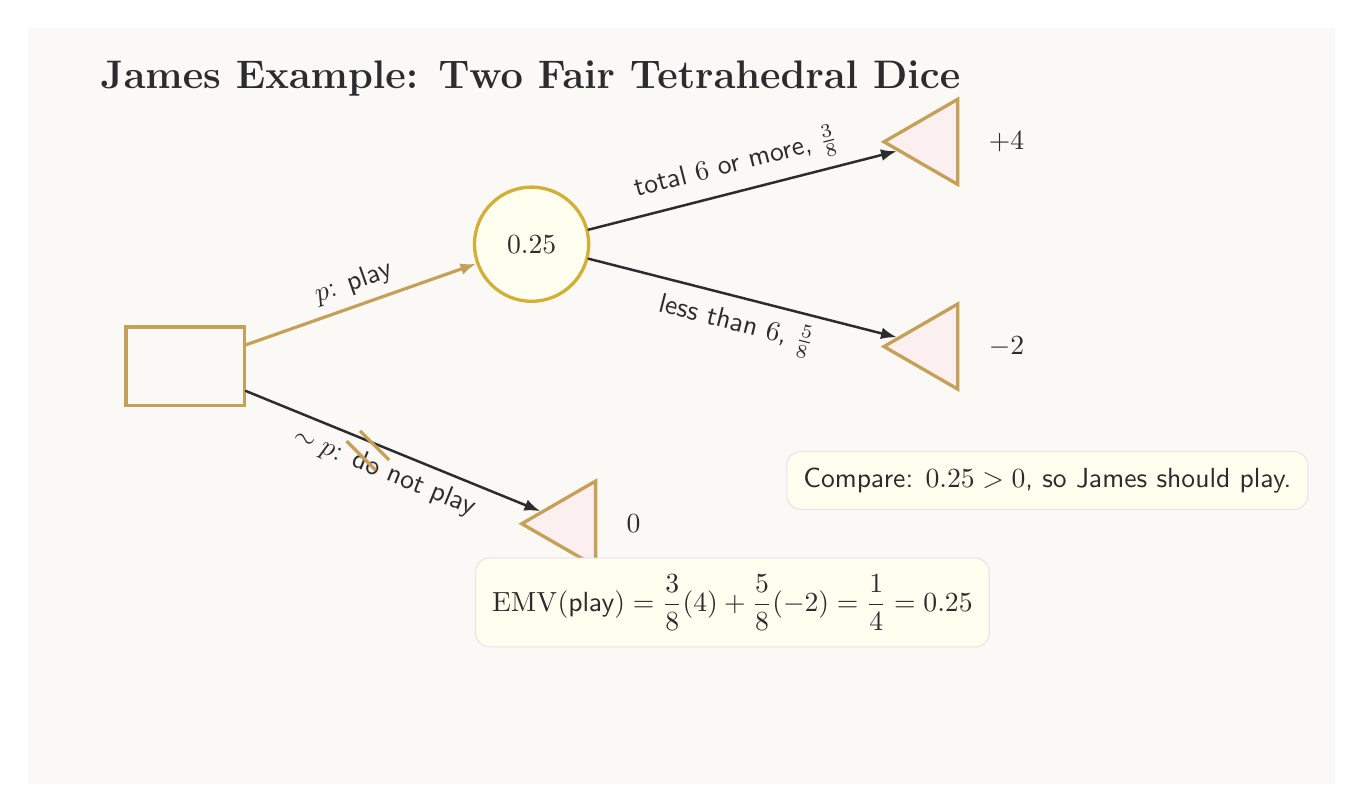
\begin{tikzpicture}[font=\sffamily,x=1cm,y=1cm]
\fill[Canvas] (-0.8,-2.2) rectangle (15.8,7.4);
\node[anchor=west,text=Ink,font=\bfseries\Large] at (0,6.75) {James Example: Two Fair Tetrahedral Dice};
\node[decision] (D0) at (1.2,3.1) {};
\node[chance] (C1) at (5.6,4.65) {$0.25$};
\node[payoff] (W) at (10.7,5.95) {};
\node[payoff] (L) at (10.7,3.35) {};
\node[payoff] (N) at (6.1,1.1) {};
\draw[chosenbranch] (D0) -- node[above,sloped,text=Ink] {$p$: play} (C1);
\draw[branch] (D0) -- node[below,sloped,text=Ink] {$\sim p$: do not play} (N);
\draw[branch] (C1) -- node[above,sloped,text=Ink] {total $6$ or more, $\frac{3}{8}$} (W);
\draw[branch] (C1) -- node[below,sloped,text=Ink] {less than $6$, $\frac{5}{8}$} (L);
\node[anchor=west,text=Ink] at ($(W.east)+(0.25,0)$) {$+4$};
\node[anchor=west,text=Ink] at ($(L.east)+(0.25,0)$) {$-2$};
\node[anchor=west,text=Ink] at ($(N.east)+(0.25,0)$) {$0$};
\draw[Gold,line width=1.2pt] (3.25,2.15)--(3.62,1.78);\draw[Gold,line width=1.2pt] (3.42,2.28)--(3.79,1.91);
\node[callout] at (8.15,0.1) {$\displaystyle \operatorname{EMV}(\text{play})=\frac{3}{8}(4)+\frac{5}{8}(-2)=\frac14=0.25$};
\node[callout] at (12.15,1.65) {Compare: $0.25>0$, so James should play.};
\end{tikzpicture}
\end{document}
